\chapter{Where is your analytics in SRA?}


Regarding on \ac{sra}, The \ac{rami} consists of a three-dimensional coordinate system containing the essential aspects of Industry 4.0. With this system the complexity between things can be reduced to more manageable units. The three axes represent all of the essential components of Industry 4.0, which consists of: Hierarchy Levels axis, Life Cycle Value Stream axis, and Layers axis \cite{Hankel2015}.

\bigskip

In the beginning, we introduced RAMI 4.0, outlining its structure and the three axes for all the crucial parts of Industry 4.0. The RAMI 4.0 model employs these three dimensions as a framework for classifying serval objects, with all critical aspects of Industry 4.0 being mapped onto them. As shown in Figure \ref{fig:Position of Analytic Application in RAMI 4.0}, we can consider the following ways to map our gait injuries prediction system to the RAMI 4.0 framework as part of our analysis of Gait Pattern Recognition using an Arduino Portenta H7 IMU:

\begin{figure}[ht]
    \centering
    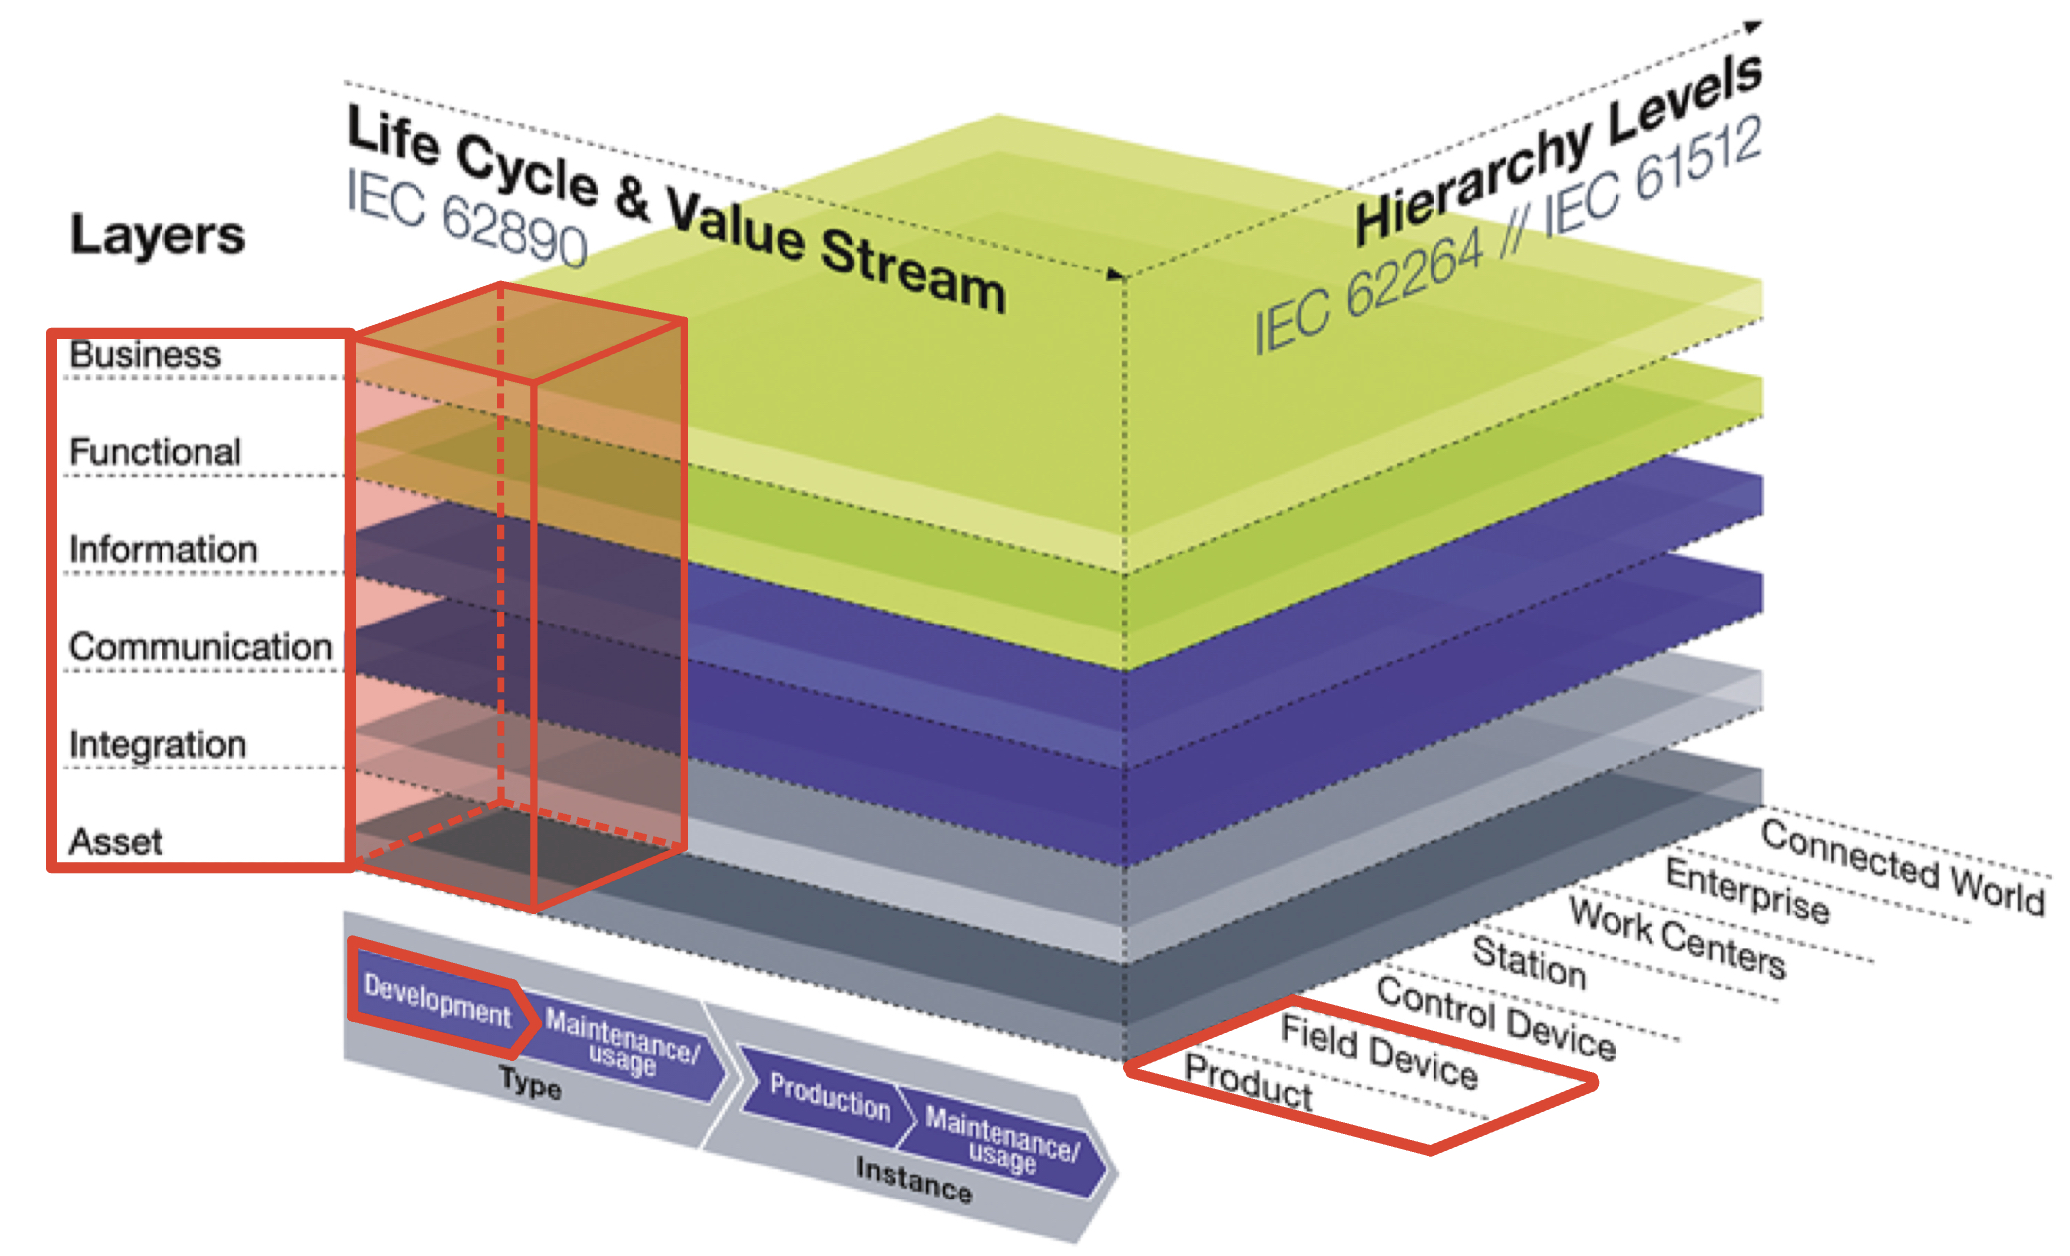
\includegraphics[scale=0.15]{Images/Position of Analytic Application in RAMI4.jpg}
    \captionsetup{justification=centering}
    \caption{Position of Analytic Application in RAMI 4.0 Based on: \cite{Hankel2015}}
    \label{fig:Position of Analytic Application in RAMI 4.0}
\end{figure}

\subsubsection{Layers axis}
\begin{itemize}
\item \textbf{Business layer}:
This layer contains the system's business context, objectives, value proposition, and stakeholders. We sell a gait injury prediction system for hospitals, rehab centers, sports teams, and senior care institutions. We could also offer subscriptions or one-time payments.

\item \textbf{Functional layer}: 
This layer contains the system's algorithms, procedures, and services. The gait injury prediction system's functional layer uses a Recurrent Neural Network (RNN) to detect and forecast gait-related injuries.

\item \textbf{Information layer}:
This layer stores and processes the system's data. The gait parameters dataset (HS, TS, HO, and TO) was obtained from the accelerometer and prepared by the Butterworth filter. The Recurrent Neural Network (RNN) will analyze this dataset to diagnose and predict injuries based on gait patterns.

\item \textbf{Communication layer}:
This layer describes the protocols and standards used by the system to communicate with other devices or systems. The communication layer of the gait injury prediction system consists of the various Bluetooth interfaces used by the Arduino Portenta H7 IMU.

\item \textbf{Integration layer}:
This layer shows how the system connects to other platforms and what standards and protocols are used. The integration layer connects the Arduino Portenta H7 IMU and the Recurrent Neural Network (RNN) training using TensorFlow lite in the gait injury prediction system (HS, TS, HO, TO).

\item \textbf{Asset layer}:
This layer contains the system's physical assets. The gait injury prediction system's asset layer includes the Arduino Portenta H7 microcontroller, the Accelerometer, the Bluetooth Module, the \ac{lipo}, and any other hardware or software.
\end{itemize}

\subsubsection{Life Cycle Value Stream axis}
As Type data, the gait injury prediction system using the Arduino Portenta H7 IMU can be seen as mapping to the Life Cycle \& Value Stream (IEC 62890) axis, which depicts the development and maintenance usage of the system.

\begin{itemize}
\item \textbf{Development}: At this point, the injury prediction system's idea and requirements are being defined. This includes the system's functions and capabilities. Moreover, the gait injury prediction system's hardware and software are also designed at this stage, including Arduino Portenta H7 microcontroller, accelerometer, algorithms, and software to diagnose and predict injuries based on gait patterns. 
\end{itemize}

\subsubsection{Hierarchy Levels axis}
\begin{itemize}
\item \textbf{Product}: Gait injuries prediction system hardware and software components, including the Arduino Portenta H7 microcontroller, Accelerometer (Inertial Measurement Unit), Bluetooth Module, Li-Po battery, and any other hardware or software used by the system, are represented at the product level.
\item \textbf{Field Product}: The field product level describes the implementation of a gait injury prediction system in the field, either as a self-contained unit or as a component of a larger, more comprehensive system or platform.
\end{itemize}